% -*- TeX-engine: luatex -*-
\documentclass[presentation,aspectratio=43,10pt]{beamer}
\usepackage{template}
\renewcommand{\authorname}{Lawrence Mitchell\inst{*}}
\renewcommand{\authoremail}{\inst{*}\texttt{lawrence.mitchell@durham.ac.uk}}

\renewcommand{\sessionnumber}{2}
\renewcommand{\sessiontitle}{Memory hierarchy}
\usepackage{tikz}
\usetikzlibrary{matrix,fit,positioning,calc}
\usepackage{pgfplots}
\pgfplotsset{compat=1.15}
\usepackage{pgfplotstable}
\date{}

\begin{document}
\begin{frame}
  \maketitle
\end{frame}


\begin{frame}
  \frametitle{Sum reduction benchmark}
  In exercise 1, you hopefully produced a plot similar to this one.

  Notice how the SIMD code has four distinct performance plateaus,
  whereas the scalar code only really has two.

  \begin{center}
    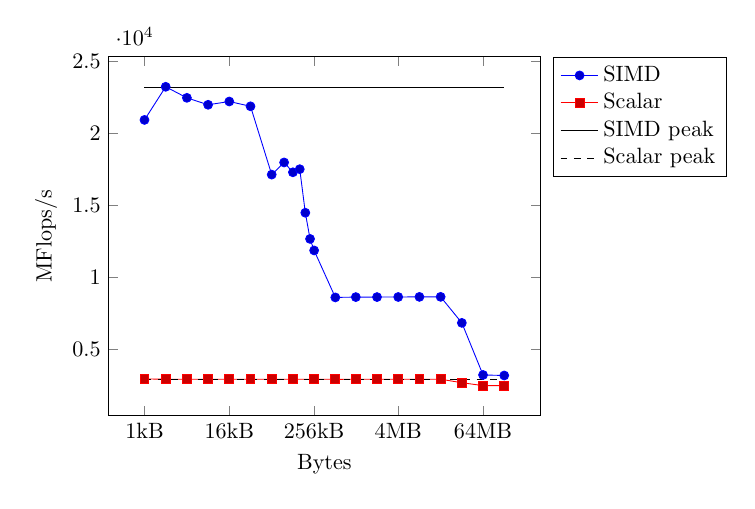
\begin{tikzpicture}[scale=0.8]
      \begin{axis}[xlabel={Bytes},
        ylabel near ticks,
        ylabel={MFlops/s},
        xmode=log,
        xtick={1e3,16e3,256e3,4e6,64e6},
        xticklabels={1kB,16kB,256kB,4MB,64MB},
        log basis x={10},
        legend pos={outer north east},
        legend style={cells={anchor=west, align=left}},]
        \pgfplotstableread[row sep=\\]{%
          Bytes MFlops Peak\\
          1e3 20934.77 23.2e3\\
          2e3 23240.25 23.2e3\\
          4e3 22471.22 23.2e3\\
          8e3 21988.17 23.2e3\\
          16e3 22216.43 23.2e3\\
          32e3 21881.05 23.2e3\\
          64e3 17130.67 23.2e3\\
          96e3 17975.12 23.2e3\\
          128e3 17291.29 23.2e3\\
          160e3 17507.30 23.2e3\\
          192e3 14476.12 23.2e3\\
          224e3 12656.81 23.2e3\\
          256e3 11854.84 23.2e3\\
          512e3 8585.19 23.2e3\\
          1e6 8607.97 23.2e3\\
          2e6 8609.45 23.2e3\\
          4e6 8615.55 23.2e3\\
          8e6 8622.28 23.2e3\\
          16e6 8624.76 23.2e3\\
          32e6 6814.45 23.2e3\\
          64e6 3190.88 23.2e3\\
          128e6 3153.69 23.2e3\\}\avxdata
        \pgfplotstableread[row sep=\\]{%
          Bytes MFlops Peak\\
          1e3 2913.70 2.9e3\\
          2e3 2893.67 2.9e3\\
          4e3 2894.32 2.9e3\\
          8e3 2894.57 2.9e3\\
          16e3 2894.35 2.9e3\\
          32e3 2889.47 2.9e3\\
          64e3 2889.47 2.9e3\\
          128e3 2891.86 2.9e3\\
          256e3 2891.90 2.9e3\\
          512e3 2887.25 2.9e3\\
          1e6 2889.04 2.9e3\\
          2e6 2888.07 2.9e3\\
          4e6 2892.18 2.9e3\\
          8e6 2892.26 2.9e3\\
          16e6 2892.14 2.9e3\\
          32e6 2651.69 2.9e3\\
          64e6 2449.17 2.9e3\\
          128e6 2445.51 2.9e3\\}\scalardata

        \addplot+ table[x=Bytes,y=MFlops] {\avxdata};
        \addlegendentry{SIMD}
        \addplot+ table[x=Bytes, y=MFlops] {\scalardata};
        \addlegendentry{Scalar}
        \addplot+[black, mark=none] table[x=Bytes, y={Peak}] {\avxdata};
        \addlegendentry {SIMD peak}
        \addplot+[black, dashed, mark=none] table[x=Bytes, y={Peak}, dashed] {\scalardata};
        \addlegendentry {Scalar peak}
      \end{axis}
    \end{tikzpicture}
  \end{center}
\end{frame}

\begin{frame}
  \frametitle{Performance peak}
  \begin{itemize}
  \item Broadwell chips can issue up to one ADD (scalar or vector) per
    cycle.
  \item Peak clock speed is 2.9GHz for this hardware.
  \end{itemize}
  \begin{challenge}{Question}
    Why does the vectorised code not achieve theoretical peak for all
    vector sizes?
  \end{challenge}
  \pause
  \begin{answer}{Lack of hardware resource}
    Recall that as well as worrying about instruction throughput, we
    have to think about data transfers.

    $\Rightarrow$ need to consider the memory hierarchy.
  \end{answer}
\end{frame}

\begin{frame}
  \frametitle{Memory hierarchy}
  \begin{columns}
    \begin{column}{0.45\textwidth}
      Can either build \emph{small} and \emph{fast} memory\\
      or\\[\baselineskip]
      \emph{large} and \emph{slow} memory.\\[\baselineskip]

      Not possible to have large and fast: physics gets in the way.
    \end{column}
    \begin{column}{0.4\textwidth}
      \begin{center}
        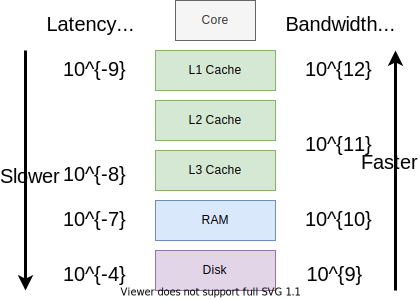
\includegraphics[width=\textwidth]{figures/cachesketch}
      \end{center}
    \end{column}
  \end{columns}
  \vspace{\baselineskip}
  $\Rightarrow$ Purpose of many optimisations is to refactor
  algorithms to keep data in fast memory.

  
  {\footnotesize See
    \url{https://colin-scott.github.io/personal_website/research/interactive_latency.html}
    for more detail on latencies}
\end{frame}

\begin{frame}
  \frametitle{Main idea for caches}
  \begin{itemize}
  \item Add hierarchy of small, fast memory.
  \item Keeps a copy of \emph{frequently used} data, speeding up
    access
  \item Typically not possible to \emph{a priori} know which data will
    be needed frequently.
  \item[$\Rightarrow$] Caches rely on \emph{princple of locality}
  \end{itemize}
\end{frame}
\begin{frame}
  \frametitle{Principle of locality}
  \begin{itemize}
  \item Normally impossible to decide before execution exactly which
    data will be needed ``frequently''.
  \item In practice, most programs (could) exhibit \emph{locality} of data
    access.
  \item Optimised algorithms will attempt to \emph{exploit} this
    locality.
  \end{itemize}

  \begin{block}{Temporal locality}
    If I access data at some memory address, it is likely that I will
    do so again ``soon''.
  \end{block}
  \begin{block}{Spatial locality}
    If I access data at some memory address, it is likely that I will
    access neighbouring addresses.
  \end{block}  
\end{frame}

\begin{frame}[fragile]
  \frametitle{Temporal locality}
  \begin{itemize}
  \item The first time we access an address, it is loaded from main
    memory \emph{and} stored in the cache.
  \item We pay a (small) penalty for the first load (storing is not free).
  \item But subsequent accesses to that address use the copy in the
    cache, and are much faster.
  \end{itemize}
  \begin{exampleblock}{Sum reduction}
\begin{minted}{c}
float s[16] = 0
for (i = 0; i < N; i++)
  s[i%16] += a[i];
\end{minted}
    Access to 16 entries of $s$ exhibits temporal locality. Makes
    sense to keep all of $s$ in cache.
  \end{exampleblock}
\end{frame}
\begin{frame}[fragile]
  \frametitle{Spatial locality}
  \begin{itemize}
  \item When accessing an address $a$, we load and store it in the
    cache.
  \item We also load and store neighbouring addresses, e.g.~$a+1$,
    $a+2$, $a+3$ \emph{at the same time}.
  \item We pay a penalty for the first load (because we're loading
    more data).
  \item Hope that next load is for $a+1$, then access will be fast.
  \end{itemize}
  \begin{exampleblock}{Sum reduction}
\begin{minted}{c}
float s[16] = 0
for (i = 0; i < N; i++)
  s[i%16] += a[i];
\end{minted}
    Access to $a$ exhibits spatial locality. Makes sense when loading
    \texttt{a[i]} to also load \texttt{a[i+1]} (it will be used in the
    next iteration).
  \end{exampleblock}
\end{frame}

\begin{frame}
  \frametitle{Designing a cache}
  \begin{block}{Important questions}
    \begin{enumerate}
    \item When we load data into the cache, where do we put it?
    \item If we have an address, how do determine if it is in the
      cache?
    \item What do we do when the cache becomes full?
    \end{enumerate}
  \end{block}

  \begin{itemize}
  \item (1) \& (2) are intimately related.
  \end{itemize}
\end{frame}

\begin{frame}[fragile]
  \frametitle{Putting data in a cache}
  \begin{itemize}
  \item Each datum uniquely referenced by its \emph{address}, $K$
    bits.  Usually $K = 32$ or $K = 64$.
  \item Need to turn this large address into a cache location.
  \end{itemize}

  \begin{block}{Direct mapped caches}
    \begin{itemize}
    \item Cache can store $2^N$ bytes.
    \item Divided into \emph{blocks} each of $2^M$ bytes.
    \item Each address references one byte.
    \item Use $N$ bits of the address, to select which slot
      in the cache to use.
    \end{itemize}
  \end{block}
\end{frame}

\begin{frame}[fragile]
  \frametitle{Direct mapped caches: indexing}
  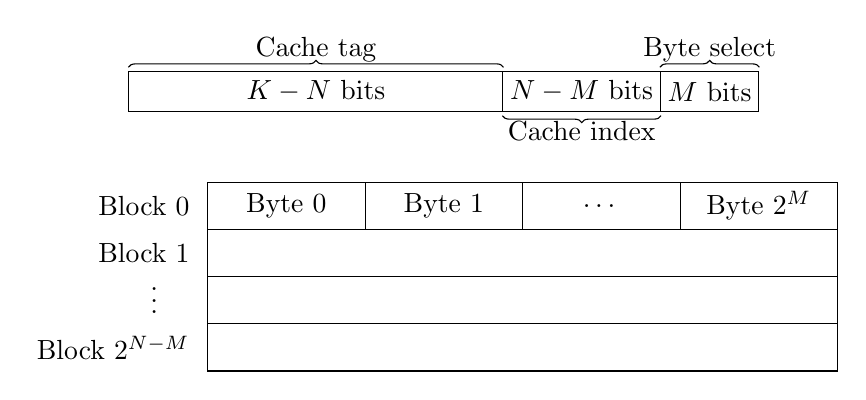
\begin{tikzpicture}
    \node[fit={(-1,1.5) (3.75, 2)}, inner sep=0pt,draw] (tag) {};
    \node at (tag.center) {$K - N$ bits};
    \draw[decoration={brace,raise=0.05cm},decorate] (tag.north west)
    -- (tag.north east) node [pos=0.5, anchor=south] {Cache tag};

    \node[fit={(3.75,1.5) (5.75, 2)}, inner sep=0pt,draw] (index) {};
    \node at (index.center) {$N-M$ bits};
    \draw[decoration={brace,raise=0.05cm},decorate] (index.south
    east) -- (index.south west) node[pos=0.5, anchor=north] {Cache index};

    \node[fit={(5.75,1.5) (7, 2)}, inner sep=0pt,draw] (select) {};
    \node at (select.center) {$M$ bits};
    \draw[decoration={brace, raise=0.05cm},decorate] (select.north west)
    -- (select.north east) node [pos=0.5, anchor=south]
    {Byte select};


    \node[fit={(0,0) (2,0.6)}, inner sep=0pt,draw] (byte0) {};
    \node at (byte0.center) {Byte 0};
    \node[fit={(2,0) (4,0.6)}, inner sep=0pt,draw] (byte1) {};
    \node at (byte1.center) {Byte 1};
    \node[fit={(4,0) (6,0.6)}, inner sep=0pt,draw] (byte2) {};
    \node at (byte2.center) {\dots};
    \node[fit={(6,0) (8,0.6)}, inner sep=0pt,draw] (byteM) {};
    \node at (byteM.center) {Byte $2^M$};

    \node[left=0.1cm of byte0] {Block 0};
    \node[fit={(0, 0) (8, -0.6)}, inner sep=0pt,draw] (block1) {};
    \node[left=0.1cm of block1] {Block 1};
    \node[fit={(0, -0.6) (8, -1.2)}, inner sep=0pt,draw] (block2) {};
    \node[left=0.5cm of block2,yshift=0.1cm] {\vdots};
    \node[fit={(0, -1.2) (8, -1.8)}, inner sep=0pt,draw] (blockN) {};
    \node[left=0.1cm of blockN] {Block $2^{N-M}$};
  \end{tikzpicture}
  \begin{itemize}
  \item \textbf{Byte select}: Use lowest $M$ bits to select correct byte in block.
  \item \textbf{Cache index}: Use next $N-M$ bits to select correct block.
  \item \textbf{Cache tag}: Use remaining $K - N$ bits as a key.
  \end{itemize}
\end{frame}

\begin{frame}
  \frametitle{Choice of block size}
  \begin{itemize}
  \item Data is loaded one \emph{block} at a time (also called \emph{cache lines}).
  \item Immediately exploits \emph{spatial locality}.
  \item Larger blocks are not always better.
  \item Almost all modern CPUs use 64byte block size.
  \end{itemize}
  \begin{corollary}
    Cache-friendly algorithms work on cache line sized chunks of data.
  \end{corollary}
\end{frame}

\begin{frame}[fragile]
  \frametitle{Direct mapped caches: eviction}
  \begin{itemize}
  \item What happens if two addresses have the same low bit pattern?
  \item We have a \emph{conflict}.
  \item Resolution: newest loaded address wins.
  \item This is a \emph{least recently used} (LRU) eviction policy.
  \end{itemize}

  \begin{block}{What can go wrong?}
    \begin{columns}
      \begin{column}{0.45\textwidth}
\begin{minted}[fontsize=\scriptsize]{c}
int a[64], b[64], r = 0;
for (int i = 0; i < 100; i++)
   for (int j = 0; j < 64; j++)
       r += a[j] + b[j];
\end{minted}
      \end{column}
      \begin{column}{0.45\textwidth}
        \begin{itemize}
        \item 1KB cache
        \item 32 byte block size
        \item So $N=10$, $M=5$.\\
          32 blocks in the cache.
        \end{itemize}
      \end{column}
    \end{columns}
  \end{block}
\end{frame}

\begin{frame}[fragile]
  \frametitle{Conflicts reduce \emph{effective} cache size}
  \begin{center}
\begin{minted}[fontsize=\tiny]{c}
for (int j = 0; j < 64; j++)
   r += a[j] + b[j];
\end{minted}
  \end{center}
  \begin{columns}
    \begin{column}{0.5\pagewidth}
      \begin{onlyenv}<1>
        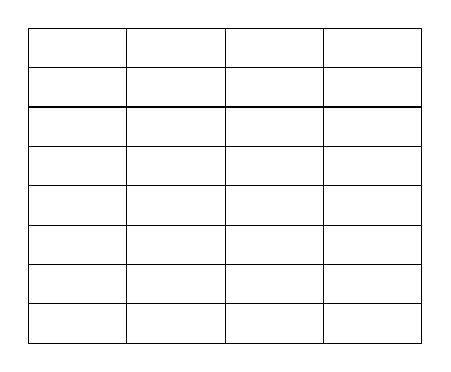
\begin{tikzpicture} [nodes in empty cells, nodes={minimum
            width=1.25cm, minimum height=0.5cm, inner sep=0}, row sep=-\pgflinewidth,
          column sep=-\pgflinewidth]
          border/.style={draw} \matrix(matrix)[matrix of nodes,
          nodes={draw}] {
            &&&\\
            &&&\\
            &&&\\
            &&&\\
            &&&\\
            &&&\\
            &&&\\
            &&&\\
          };
        \end{tikzpicture}
      \end{onlyenv}%
      \begin{onlyenv}<2>
        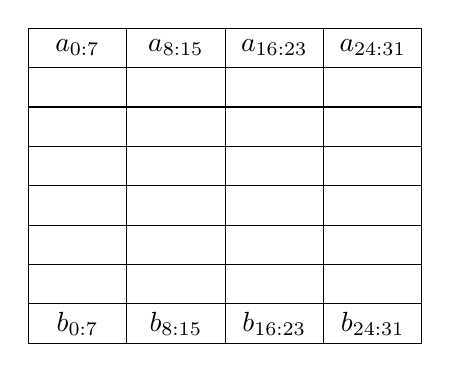
\begin{tikzpicture} [nodes in empty cells, nodes={minimum
            width=1.25cm, minimum height=0.5cm, inner sep=0}, row
          sep=-\pgflinewidth, column sep=-\pgflinewidth]
          border/.style={draw} \matrix(matrix)[matrix of nodes,
          nodes={draw}] {
            $a_{0:7}$ & $a_{8:15}$ & $a_{16:23}$ & $a_{24:31}$ \\
                      &            &             &             \\
                      &            &             &             \\
                      &            &             &             \\
                      &            &             &             \\
                      &            &             &             \\
                      &            &             &             \\
            $b_{0:7}$ & $b_{8:15}$ & $b_{16:23}$ & $b_{24:31}$ \\
          };
        \end{tikzpicture}
      \end{onlyenv}%
      \begin{onlyenv}<3>
        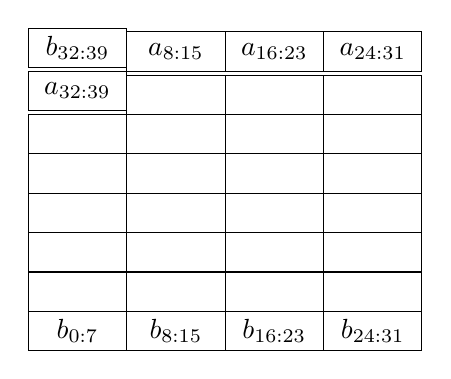
\begin{tikzpicture} [nodes in empty cells, nodes={minimum
            width=1.25cm, minimum height=0.5cm, inner sep=0}, row
          sep=-\pgflinewidth, column sep=-\pgflinewidth]
          border/.style={draw} \matrix(matrix)[matrix of nodes,
          nodes={draw}] {
            $b_{32:39}$ & $a_{8:15}$ & $a_{16:23}$ & $a_{24:31}$ \\
            $a_{32:39}$ &            &             &             \\
                        &            &             &             \\
                        &            &             &             \\
                        &            &             &             \\
                        &            &             &             \\
                        &            &             &             \\
            $b_{0:7}$   & $b_{8:15}$ & $b_{16:23}$ & $b_{24:31}$ \\
          };
        \end{tikzpicture}
      \end{onlyenv}%
      \begin{onlyenv}<4>
        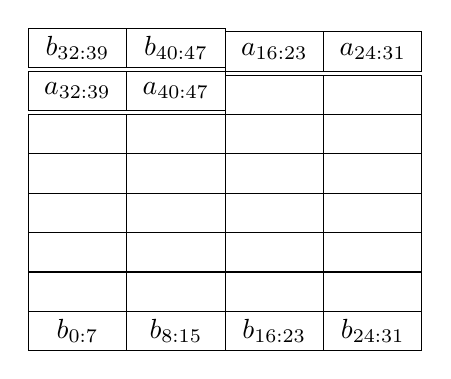
\begin{tikzpicture} [nodes in empty cells, nodes={minimum
            width=1.25cm, minimum height=0.5cm, inner sep=0}, row
          sep=-\pgflinewidth, column sep=-\pgflinewidth]
          border/.style={draw} \matrix(matrix)[matrix of nodes,
          nodes={draw}] {
            $b_{32:39}$ & $b_{40:47}$  & $a_{16:23}$ & $a_{24:31}$ \\
            $a_{32:39}$ & $a_{40:47}$ &  &  \\
                        &             &             &             \\
                        &             &             &             \\
                        &             &             &             \\
                        &             &             &             \\
                        &             &             &             \\
            $b_{0:7}$   & $b_{8:15}$  & $b_{16:23}$ & $b_{24:31}$ \\
          };
        \end{tikzpicture}
      \end{onlyenv}%
      \begin{onlyenv}<5>
        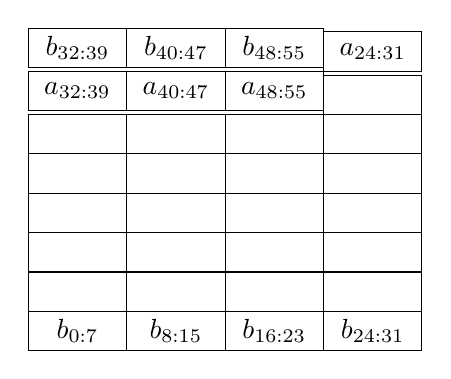
\begin{tikzpicture} [nodes in empty cells, nodes={minimum
            width=1.25cm, minimum height=0.5cm, inner sep=0}, row
          sep=-\pgflinewidth, column sep=-\pgflinewidth]
          border/.style={draw} \matrix(matrix)[matrix of nodes,
          nodes={draw}] {
            $b_{32:39}$ & $b_{40:47}$ & $b_{48:55}$ & $a_{24:31}$ \\
            $a_{32:39}$ & $a_{40:47}$ & $a_{48:55}$ &             \\
                        &             &             &             \\
                        &             &             &             \\
                        &             &             &             \\
                        &             &             &             \\
                        &             &             &             \\
            $b_{0:7}$   & $b_{8:15}$  & $b_{16:23}$ & $b_{24:31}$ \\
          };
        \end{tikzpicture}
      \end{onlyenv}%
      \begin{onlyenv}<6->
        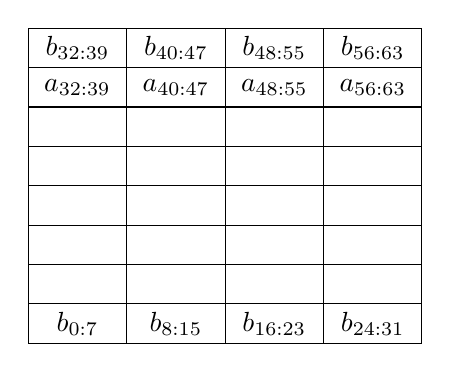
\begin{tikzpicture} [nodes in empty cells, nodes={minimum
            width=1.25cm, minimum height=0.5cm, inner sep=0}, row
          sep=-\pgflinewidth, column sep=-\pgflinewidth]
          border/.style={draw} \matrix(matrix)[matrix of nodes,
          nodes={draw}] {
            $b_{32:39}$ & $b_{40:47}$ & $b_{48:55}$ & $b_{56:63}$ \\
            $a_{32:39}$ & $a_{40:47}$ & $a_{48:55}$ & $a_{56:63}$ \\
                        &             &             &             \\
                        &             &             &             \\
                        &             &             &             \\
                        &             &             &             \\
                        &             &             &             \\
            $b_{0:7}$   & $b_{8:15}$  & $b_{16:23}$ & $b_{24:31}$ \\
          };
        \end{tikzpicture}
      \end{onlyenv}%
    \end{column}
    \begin{column}{0.45\pagewidth}
\begin{minted}[fontsize=\tiny]{c}
&a[00] = b..._00000_00000 => line 0, byte offset 0
&a[01] = b..._00000_00100 => line 0, byte offset 4
&a[02] = b..._00000_01000 => line 0, byte offset 8
&a[03] = b..._00000_01100 => line 0, byte offset 12
&a[04] = b..._00000_10000 => line 0, byte offset 16
&a[05] = b..._00000_10100 => line 0, byte offset 20
&a[06] = b..._00000_11000 => line 0, byte offset 24
&a[07] = b..._00000_11100 => line 0, byte offset 28
...
&b[00] = b..._11100_00000 => line 28, byte offset 0
&b[01] = b..._11100_00100 => line 28, byte offset 4
&b[02] = b..._11100_01000 => line 28, byte offset 8
&b[03] = b..._11100_01100 => line 28, byte offset 12
&b[04] = b..._11100_10000 => line 28, byte offset 16
&b[05] = b..._11100_10100 => line 28, byte offset 20
&b[06] = b..._11100_11000 => line 28, byte offset 24
&b[07] = b..._11100_11100 => line 28, byte offset 28
...
\end{minted}
    \end{column}
  \end{columns}
\end{frame}
\begin{frame}[fragile]
  \frametitle{Cache thrashing}
  \begin{block}{What can go wrong?}
    \begin{columns}
      \begin{column}{0.45\textwidth}
\begin{minted}[fontsize=\scriptsize]{c}
int A[64], B[64], r = 0;
for (int i = 0; i < 100; i++)
   for (int j = 0; j < 64; j++)
       r += A[j] + B[j];
\end{minted}
      \end{column}
      \begin{column}{0.45\textwidth}
        \begin{itemize}
        \item 1KB cache
        \item 32 byte block size
        \item So $N=10$, $M=5$. \\32 blocks in the cache.
        \end{itemize}
      \end{column}
    \end{columns}
  \end{block}

  \begin{block}{Cache thrashing}
    \begin{itemize}
    \item We need $2 \cdot 64 \cdot 4 = 512\text{ bytes}$ to store $A$
      and $B$ in cache.  This only requires 16 blocks, so our cache is
      large enough.
    \item But if the addresses match in the low bits, we will try and
      store to same locations.
    \item In worst case, every load of \texttt{B[j]} evicts
      \texttt{A[j]}, and vice versa.
    \end{itemize}
  \end{block}
\end{frame}

\begin{frame}[t]
  \frametitle{Cache associativity}
  \begin{columns}
    \begin{column}{0.48\textwidth}
      \begin{block}{Direct mapped}
        \begin{itemize}
        \item Each block from main memory maps to exactly one cache
          line.
        \item LRU eviction policy (new data overwrite old).
        \end{itemize}
      \end{block}
      \end{column}
      \begin{column}{0.48\textwidth}
        \begin{block}{Fully associative}
          \begin{itemize}
          \item Each byte from main memory can maps to any cache line.
          \item Most flexible, but also expensive.
          \end{itemize}
        \end{block}
      \end{column}
  \end{columns}
  \begin{block}{$k$-way set associative}
    \begin{itemize}
    \item $k$ ``copies'' of a direct mapped cache.  Each block from main
      memory maps to one of $k$ cache lines, called \emph{sets}.
    \item Typically use LRU eviction.
    \item Usual choice: $N \in \{2, 4, 8, 16\}$.
    \item Skylake has $N = 8$ for L1, $N = 16$ for L2, $N = 11$
      for L3.
    \end{itemize}
  \end{block}
\end{frame}


\begin{frame}
  \frametitle{Exercise: cache bandwidth}
  \begin{itemize}
  \item Let's try and do this in the round again.

  \item Goal is to benchmark the memory bandwidth as a function of
    vector size to see what we observe.
  \item We will use the results to explain the observations of the sum
    reduction benchmark.
  \item[$\Rightarrow$] over to you.
  \end{itemize}
  \begin{center}
    \url{teaching.wence.uk/comp52315/exercises/exercise02/}
  \end{center}
\end{frame}

\begin{frame}
  \frametitle{Results}
  You hopefully produced a plot similar to this one.

  I added the floating point throughtput of the sum reduction so we
  can compare the plateaus.
  \begin{center}
    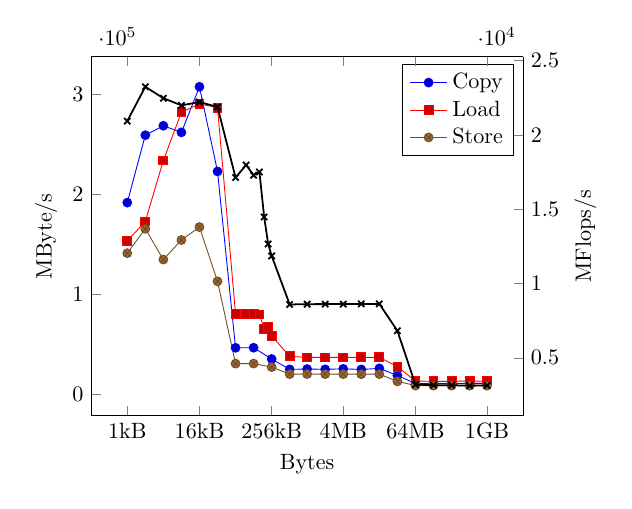
\begin{tikzpicture}[scale=0.8]
      \begin{axis}[xlabel={Bytes},
        ylabel near ticks,
        axis y line*=left,
        ylabel={MByte/s},
        xmode=log,
        xtick={1e3,16e3,256e3,4e6,64e6,1e9},
        xticklabels={1kB,16kB,256kB,4MB,64MB,1GB},
        log basis x={10},
        legend style={cells={anchor=west, align=left}},]
        \pgfplotstableread[row sep=\\]{%
          Bytes MBytes\\
          1e3 191682.87\\
          2e3 259178.92\\
          4e3 268609.79\\
          8e3 262007.62\\
          16e3 307619.45\\
          32e3 222883.57\\
          64e3 46327.33\\
          128e3 46415.36\\
          256e3 35150.15\\
          512e3 24771.07\\
          1e6 25080.55\\
          2e6 24812.26\\
          4e6 25289.10\\
          8e6 24673.00\\
          16e6 25747.47\\
          32e6 18618.29\\
          64e6 10630.21\\
          128e6 10639.17\\
          256e6 10502.63\\
          512e6 10690.16\\
          1e9 10819.48\\
        }\copy
        \pgfplotstableread[row sep=\\]{%
          Bytes MBytes\\
          1e3 153340.47\\
          2e3 172851.18\\
          4e3 233932.86\\
          8e3 282139.80\\
          16e3 290516.79\\
          32e3 286756.91\\
          64e3 80135.26\\
          96e3 80391.69\\
          128e3 79891.71\\
          160e3 79719.73\\
          192e3 65256.46\\
          224e3 67087.59\\
          256e3 58293.14\\
          512e3 37787.61\\
          1e6 36722.61\\
          2e6 36763.74\\
          4e6 36675.27\\
          8e6 36793.72\\
          16e6 36816.49\\
          32e6 27525.82\\
          64e6 13075.06\\
          128e6 12781.75\\
          256e6 12806.85\\
          512e6 13083.85\\
          1e9 12788.69\\
        }\load
        \pgfplotstableread[row sep=\\]{%
          Bytes MBytes\\
          1e3 141087.63\\
          2e3 165450.51\\
          4e3 134665.13\\
          8e3 154274.23\\
          16e3 167200.39\\
          32e3 112887.10\\
          64e3 30526.56\\
          128e3 30539.02\\
          256e3 27057.18\\
          512e3 20037.34\\
          1e6 20027.31\\
          2e6 20012.49\\
          4e6 20000.02\\
          8e6 19903.02\\
          16e6 20008.66\\
          32e6 12723.63\\
          64e6 8568.50\\
          128e6 8497.95\\
          256e6 8441.10\\
          512e6 8457.19\\
          1e9 8486.48\\
        }\store
        \addplot+ table[x=Bytes,y=MBytes] {\copy};
        \addlegendentry{Copy}
        \addplot+ table[x=Bytes,y=MBytes] {\load};
        \addlegendentry{Load}
        \addplot+ table[x=Bytes,y=MBytes] {\store};
        \addlegendentry{Store}
      \end{axis}
      \pause
      \begin{axis}[xlabel={},
        ylabel near ticks,
        axis y line*=right,
        ylabel={MFlops/s},
        xmode=log,
        xtick={1e3,16e3,256e3,4e6,64e6,1e9},
        xticklabels={},
        log basis x={10},
        legend pos={outer north east},
        legend style={cells={anchor=west, align=left}},]
        \pgfplotstableread[row sep=\\]{%
          Bytes MFlops Peak\\
          1e3 20934.77 23.2e3\\
          2e3 23240.25 23.2e3\\
          4e3 22471.22 23.2e3\\
          8e3 21988.17 23.2e3\\
          16e3 22216.43 23.2e3\\
          32e3 21881.05 23.2e3\\
          64e3 17130.67 23.2e3\\
          96e3 17975.12 23.2e3\\
          128e3 17291.29 23.2e3\\
          160e3 17507.30 23.2e3\\
          192e3 14476.12 23.2e3\\
          224e3 12656.81 23.2e3\\
          256e3 11854.84 23.2e3\\
          512e3 8585.19 23.2e3\\
          1e6 8607.97 23.2e3\\
          2e6 8609.45 23.2e3\\
          4e6 8615.55 23.2e3\\
          8e6 8622.28 23.2e3\\
          16e6 8624.76 23.2e3\\
          32e6 6814.45 23.2e3\\
          64e6 3190.88 23.2e3\\
          128e6 3153.69 23.2e3\\
          256e6 3150.00 23.2e3\\
          512e6 3120.00 23.2e3\\
          1e9 3130.00 23.2e3\\}\avxdata
        \addplot+[black, mark=x, thick] table[x=Bytes,y=MFlops] {\avxdata};
      \end{axis}
    \end{tikzpicture}
  \end{center}
\end{frame}

\begin{frame}
  \frametitle{Interpretation}
  \begin{itemize}
  \item Vectorised addition requires 1 32Byte load/cycle (for the 8
    floats)
  \item Accumulation parameter held in a register.
  \item[$\Rightarrow$] requires sustained load bandwidth of $32\times
    2.9 = 92.8$GByte/s
  \item From L1 (less than 32kB) we see sustained bandwidth of around
    300GByte/s $\Rightarrow$ floating-point throughput is limit.
  \item L2 (less than 256kB) provides around 80GByte/s or around
    27Bytes/cycle $\Rightarrow$ 6.75 floats/cycle $\Rightarrow$ peak
    is around 19GFlops/s.
  \item L3 (less than 30MB) provides around 36GByte/s or around
    12Bytes/cycle $\Rightarrow$ 2.75 floats/cycle $\Rightarrow$ peak
    is around 8GFlops/s.
  \item Main memory provides around 13GByte/s or around 4.5Bytes/cycle
    $\Rightarrow$ 1.1floats/cycle $\Rightarrow$ peak is around 3.25GFlops/s.
  \end{itemize}
\end{frame}

\begin{frame}
  \frametitle{Adding bandwidth-induced limits}
  Not bad for a pen-and-paper exercise.
  \begin{center}
    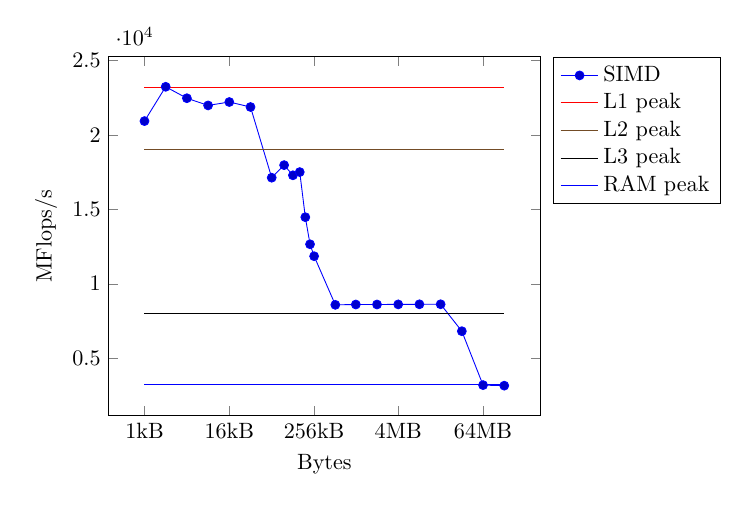
\begin{tikzpicture}[scale=0.8]
      \begin{axis}[xlabel={Bytes},
        ylabel near ticks,
        ylabel={MFlops/s},
        xmode=log,
        xtick={1e3,16e3,256e3,4e6,64e6},
        xticklabels={1kB,16kB,256kB,4MB,64MB},
        log basis x={10},
        legend pos={outer north east},
        legend style={cells={anchor=west, align=left}},]
        \pgfplotstableread[row sep=\\]{%
          Bytes MFlops Peak L2Peak L3Peak RAMPeak\\
          1e3 20934.77 23.2e3 19e3 8e3 3.25e3\\
          2e3 23240.25 23.2e3 19e3 8e3 3.25e3\\
          4e3 22471.22 23.2e3 19e3 8e3 3.25e3\\
          8e3 21988.17 23.2e3 19e3 8e3 3.25e3\\
          16e3 22216.43 23.2e3 19e3 8e3 3.25e3\\
          32e3 21881.05 23.2e3 19e3 8e3 3.25e3\\
          64e3 17130.67 23.2e3 19e3 8e3 3.25e3\\
          96e3 17975.12 23.2e3 19e3 8e3 3.25e3\\
          128e3 17291.29 23.2e3 19e3 8e3 3.25e3\\
          160e3 17507.30 23.2e3 19e3 8e3 3.25e3\\
          192e3 14476.12 23.2e3 19e3 8e3 3.25e3\\
          224e3 12656.81 23.2e3 19e3 8e3 3.25e3\\
          256e3 11854.84 23.2e3 19e3 8e3 3.25e3\\
          512e3 8585.19 23.2e3 19e3 8e3 3.25e3\\
          1e6 8607.97 23.2e3 19e3 8e3 3.25e3\\
          2e6 8609.45 23.2e3 19e3 8e3 3.25e3\\
          4e6 8615.55 23.2e3 19e3 8e3 3.25e3\\
          8e6 8622.28 23.2e3 19e3 8e3 3.25e3\\
          16e6 8624.76 23.2e3 19e3 8e3 3.25e3\\
          32e6 6814.45 23.2e3 19e3 8e3 3.25e3\\
          64e6 3190.88 23.2e3 19e3 8e3 3.25e3\\
          128e6 3153.69 23.2e3 19e3 8e3 3.25e3\\}\avxdata
        \addplot+ table[x=Bytes,y=MFlops] {\avxdata};
        \addlegendentry{SIMD}
        \addplot+[mark=none] table[x=Bytes, y={Peak}] {\avxdata};
        \addlegendentry {L1 peak}
        \addplot+[mark=none] table[x=Bytes, y={L2Peak}] {\avxdata};
        \addlegendentry {L2 peak}
        \addplot+[mark=none] table[x=Bytes, y={L3Peak}] {\avxdata};
        \addlegendentry {L3 peak}
        \addplot+[mark=none] table[x=Bytes, y={RAMPeak}] {\avxdata};
        \addlegendentry {RAM peak}
      \end{axis}
    \end{tikzpicture}
  \end{center}
\end{frame}
\begin{frame}
  \frametitle{Memory/node topology}
  \texttt{likwid-topology} reports an ASCII version of diagrams like
  this.
  \begin{center}
    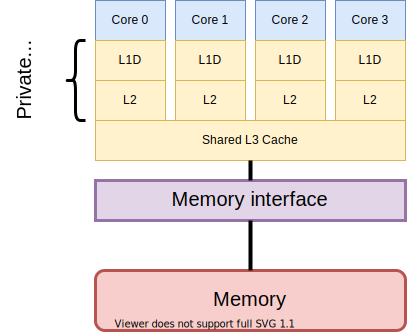
\includegraphics[height=0.5\textheight]{figures/cacheschematic}
  \end{center}
\end{frame}

\begin{frame}
  \frametitle{More than one core}
  \begin{itemize}
  \item So far, just looked at performance when we use a single core.
  \item In practice, most scientific computing algorithms will be
    parallel
  \item[$\Rightarrow$] How does this affect the performance?
  \end{itemize}

  \begin{answer}{Scalable vs.~Saturating}
    CPU cores are a \emph{scalable} resource.

    Adding a second core doubles the number of floating point
    operations we can perform.

    Memory bandwidth is a \emph{saturating resource}. Outside of L2
    cache (L3, main memory), CPU cores compete for the same resource.
  \end{answer}
\end{frame}

\begin{frame}
  \frametitle{Scalable vs.~Saturating}
  \begin{columns}
    \begin{column}{0.45\textwidth}
      Shared resources might show saturating performance
      \begin{tikzpicture}
        \pgfplotstableread[row sep=\\]{%
          Cores Perf\\
          1 3\\
          2 6\\
          3 8\\
          4 9\\
          5 9.4\\
          6 9.5\\
          7 9.55\\
          8 9.56\\}\saturating
        \begin{axis}[xlabel=Cores,
          ylabel=Performance,
          width=\textwidth,height=0.7\textheight]
          \addplot+ table[x=Cores, y=Perf] {\saturating};
        \end{axis}
      \end{tikzpicture}
    \end{column}
    \begin{column}{0.45\textwidth}
      Parallel resources show scalable performance
      \begin{tikzpicture}
        \pgfplotstableread[row sep=\\]{%
          Cores Perf\\
          1 1.5\\
          2 3\\
          3 4.5\\
          4 6\\
          5 7.5\\
          6 9\\
          7 10.5\\
          8 12\\}\scaling
        \begin{axis}[xlabel=Cores,
          ylabel=Performance,
          width=\textwidth,height=0.7\textheight]
          \addplot+ table[x=Cores, y=Perf] {\scaling};
        \end{axis}
      \end{tikzpicture}
    \end{column}
  \end{columns}
\end{frame}

\begin{frame}
  \frametitle{Exercise: memory bandwidth saturation}
  \begin{itemize}
  \item Goal is to benchmark the memory bandwidth for different vector
    sizes as a function of number of cores
  \item Will then look at scaling of sum reduction with cores
  \item[$\Rightarrow$] over to you.
  \end{itemize}
  \begin{center}
    Exercises at

    \url{teaching.wence.uk/comp52315/exercises/exercise03/}
  \end{center}
\end{frame}

\begin{frame}
  \frametitle{Conclusions on hardware architecture}
  \begin{challenge}{Performance considerations}
    \begin{itemize}
    \item How many instructions are required to implement an algorithm
    \item How efficiently those instructions are executed on a
      processor
    \item The runtime contribution of the data transfers
    \end{itemize}
  \end{challenge}
  \begin{answer}{Complex ``topology'' of hardware}
    \begin{itemize}
    \item Many layers of parallelism in modern hardware
    \item Sockets: around 1-4 CPUs on a typical motherboard
    \item Cores: around 4-32 cores in a typical CPU
    \item SIMD/Vectorisation: typically 2-16 single precision elements
      in vector registers on CPUs
    \item Superscalar execution: typically 2-8 instructions per cycle
    \end{itemize}
  \end{answer}
\end{frame}
\begin{frame}
  \frametitle{Challenges for program development}
  \begin{itemize}
  \item We will focus most of our efforts on SIMD and some superscalar
    execution here.
  \item An ongoing challenge is that most programming models do not
    offer a lot of explicit access to parallelism.
  \item[$\Rightarrow$] will look at mechanisms to convince compilers
    to ``do the right thing''.
  \end{itemize}
\end{frame}
\end{document}
